\problemname{\problemyamlname}
\illustration{0.32}{congestion}{Jam caused by parking bus, \href{https://commons.wikimedia.org/wiki/File:Moscow_traffic_congestion.JPG}{Nevermind2}\vspace{-0.5cm}}%
You are the new minister of transport in Berland.
Recently, you allowed free parking on a two lane road segment of $200$ metres length.
Since then, that road segment has constantly been jammed by parked cars due to some
genius drivers who had the idea to park their cars across both lanes\dots

However, this is not your concern.
You are more interested in parking some of your own cars on the road segment while it is empty.
More specifically, you want to park some of your cars in such a way that the number of different ways to fill the remaining empty space with cars is congruent to your lucky number $n$ modulo~$10^9+7$.


\begin{figure}[h]
	\centering
	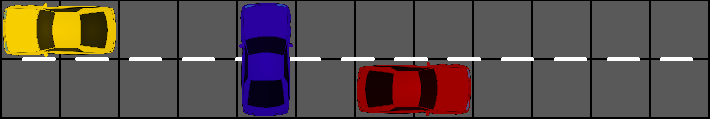
\includegraphics{sample}
	\caption{Visualization of Sample Output 1.}
\end{figure}

Each car has a size of~$1\times2$ metres, each of the two lanes is $1$ metre wide and $200$ metres long.
You own more than $200$ cars which you could park on the road segment.

\begin{Input}
	The input consists of:
	\begin{itemize}
		\item One line with one integer $n$ ($0\leq n<10^9+7$), the desired number of possible ways to fill the road modulo~$10^9+7$.
	\end{itemize}
	It can be proven that at least one valid solution exists for each possible value of~$n$.
\end{Input}

\begin{Output}
	Output the state of the two lanes in two lines.
	Print ``\texttt{\#}'' for an occupied spot and ``\texttt{.}'' for an empty spot.
	Note that the two lines should have the same length of at least $1$ metre and at most $200$ metres,
        and the occupied spots must correspond to some parked cars.
	If your solution uses a road segment shorter than $200$ metres,
        the remaining part of the road segment is assumed to be blocked by parked cars. 
\end{Output}
